\documentclass{beamer}
\mode<presentation>
{
	%\usetheme{CambridgeUS}
	\usetheme{Madrid}
	\usecolortheme{default}
	\usefonttheme{serif}
}
\usepackage[utf8]{inputenc}
\usepackage[russian]{babel}
\usepackage{cmap}
\usepackage{listings}
\usepackage{lmodern}
\usepackage{color}
\usepackage{minted}
\usepackage{graphicx}
\usepackage{tikz}
\usepackage{wrapfig}

\begin{document}
\title
[Project presentation]
{Project presentation}
\author
[Podkopaev Anton]{Podkopaev Anton, \texttt podkoav239@gmail.com}
\date [30-11-12]{30 November 2012}

\begin{frame}[plain]
	\titlepage
\end{frame}

\begin{frame}{What is project theme?}
	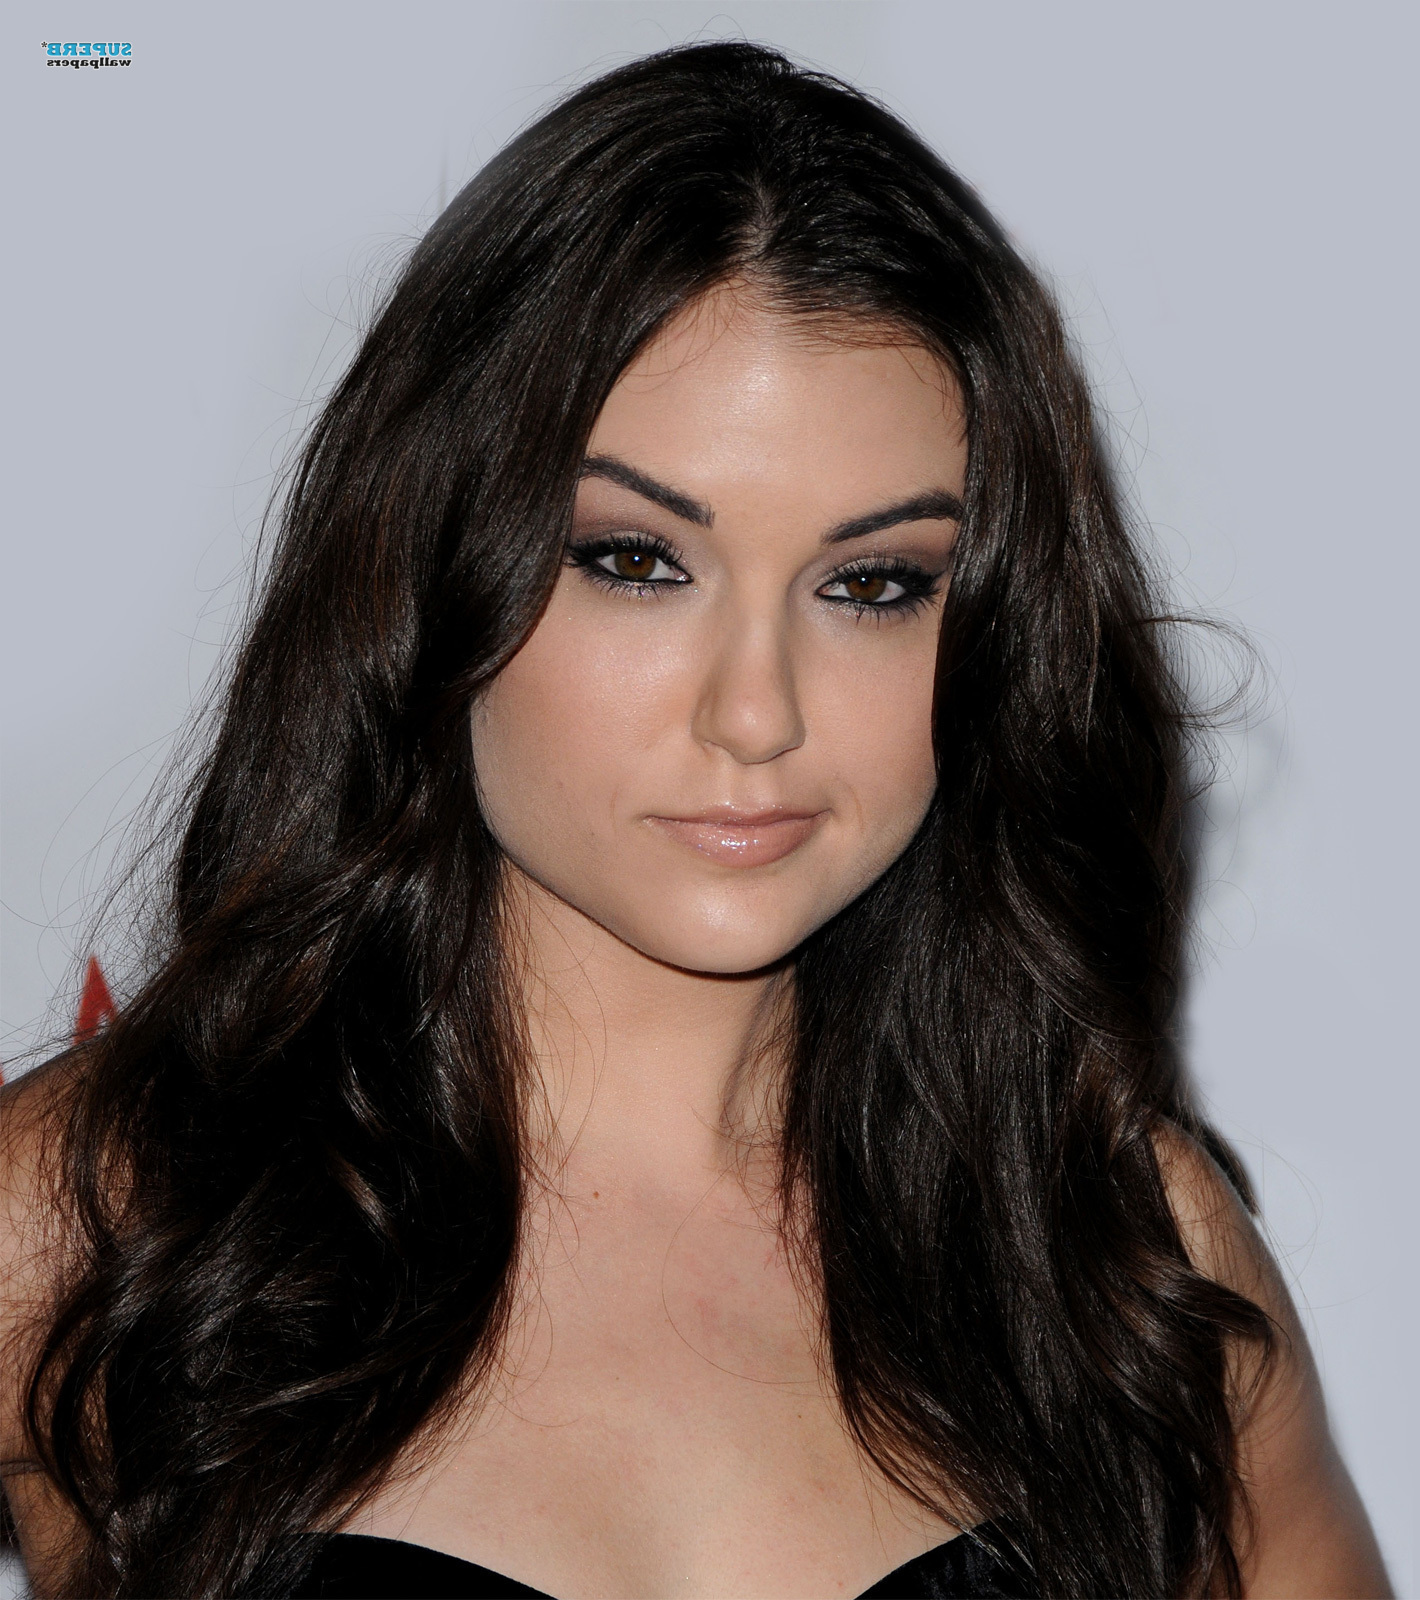
\includegraphics[width = 0.4\linewidth]{images/pretty.jpg}
	\hfill
	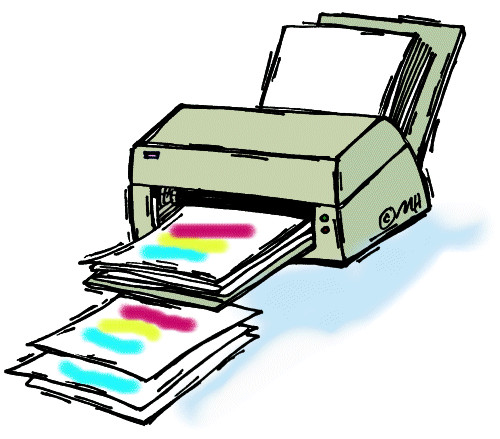
\includegraphics[width = 0.4\linewidth]{images/printing.jpg}
	\begin{center}
		Pretty-Printing
	\end{center}
\end{frame}

\begin{frame}{Pretty-Printing}
	
\includegraphics[width = 0.4\linewidth]{images/tree.jpg}
	\hfill
	
\includegraphics[width = 0.4\linewidth]{images/text.png}
\end{frame}

\begin{frame}[fragile]{Multiple layouts (1)}
	\begin{block}{}
		\inputminted{pascal}{code/for1.pas}
	\end{block}
	\begin{block}{}
		\inputminted{pascal}{code/for2.pas}
	\end{block}
\end{frame}

\begin{frame}[fragile]{Multiple layouts (2)}
	\begin{block}{}
		\inputminted{pascal}{code/if1.pas}
	\end{block}
	\begin{block}{}
		\inputminted{pascal}{code/if2.pas}
	\end{block}
	\begin{block}{}
		\inputminted{pascal}{code/if3.pas}
	\end{block}
\end{frame}

\begin{frame}{Combinators}
	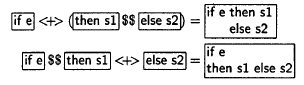
\includegraphics[width = 1\linewidth]{images/a1.png}
	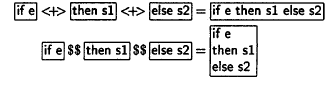
\includegraphics[width = 1\linewidth]{images/a2.png}	
\end{frame}

\begin{frame}{Problems}
	\begin{itemize}
		\item Prettiness
		\item Convenience
		\item Speed
		\vfill
		\item Optimality
	\end{itemize}
	\hfill
	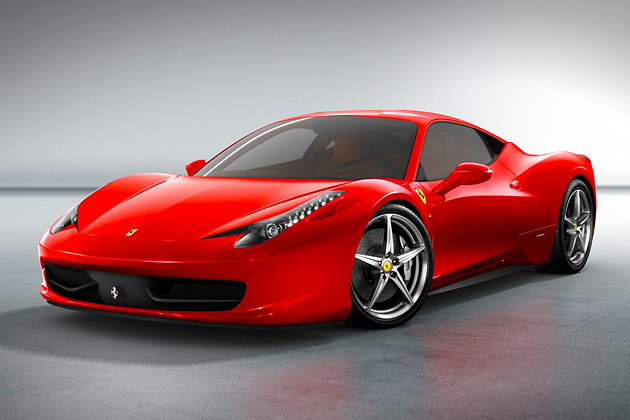
\includegraphics[width = 0.6\linewidth]{images/ferrari.jpg}
\end{frame}

\begin{frame}{Work direction}
	\begin{block}{}
		\inputminted{c}{code/while1.c}
	\end{block}
	\begin{block}{}
		\inputminted{c}{code/while2.c}
	\end{block}
	\begin{block}{}
		\inputminted{c}{code/while3.c}
	\end{block}
	\begin{block}{}
		\inputminted{c}{code/while4.c}
	\end{block}
\end{frame}

% \begin{frame}{Work direction (1)}
% 	% \begin{block}{Tree part}
% 	% 	\inputminted{haskell}{code/whileOp.hs}
% 	% \end{block}
% 	\begin{block}{}
% 		while (
% 		\begin{tikzpicture}
% 			\draw (0, 0) rectangle (1, 0.3);
% 		\end{tikzpicture}
% 		)
% 		\begin{tikzpicture}
% 			\draw (0, 0) rectangle (1, 0.3);
% 		\end{tikzpicture}		
% 	\end{block}

% 	\begin{block}{}
% 		while (
% 		\begin{tikzpicture}
% 			\draw (0, 0) rectangle (1, 0.8);
% 		\end{tikzpicture}
% 		)
% 		\begin{tikzpicture}
% 			\draw (0, 0) rectangle (1, 0.3);
% 		\end{tikzpicture}
% 	\end{block}

% 	\begin{block}{}
% 		while (
% 		\begin{tikzpicture}
% 			\draw (0, 0) rectangle (1, 0.8);
% 		\end{tikzpicture}
% 		)
% 		\newline
% 		\begin{tikzpicture}
% 			\draw (0, 0) rectangle (1, 0.8);
% 		\end{tikzpicture}
% 	\end{block}

% 	\begin{block}{}
% 		while (
% 		\begin{tikzpicture}
% 			\draw (0, 0) rectangle (1, 0.8);
% 		\end{tikzpicture}
% 		) \{
% 		\newline
% 		\begin{tikzpicture}
% 			\draw (0, 0) rectangle (1, 0.8);
% 		\end{tikzpicture}
% 		\newline
% 		\}
% 	\end{block}

% \end{frame}

\end{document}

